% 第4章第2节：集合函数的性质（单调性；模性；次模性与超模性）。

\section{集合函数的性质}
\label{sec:graph-set-function-properties}

上一节的三个例子在“加入一个元素会怎样改变评价”这个问题上表现不同：加入传感器不会减少覆盖，但可能增加的覆盖越来越少；加入一项成本总是增加固定的数额；把一个顶点移到$S$一侧，割权可能增加也可能减少。本节把这些表现分别写成单调性、模性和次模性，并说明三者各有条件，不能互相推出。

\subsection{单调性}
\label{sec:graph-setfn-monotonicity}

多装一个传感器，覆盖的格子只会增加或保持不变。把这一性质写成子集之间的比较，就是下面的定义。

\begin{definition}[单调非减]
\label{def:graph-setfn-monotone}
若对任意$A\subseteq B\subseteq V$都有$F(A)\leq F(B)$，称集合函数$F$\term{单调非减}（monotone nondecreasing），简称单调。
\end{definition}

定义比较的是任意两个有包含关系的子集，检查起来要考虑很多对。借助式~\eqref{eq:graph-setfn-telescoping}，它可以化成只检查单个元素的条件：$F$单调，当且仅当对每个$S\subseteq V$和每个$v\notin S$都有$\Delta(v\mid S)\geq0$。必要性只需取$A=S$、$B=S\cup\{v\}$。充分性：对任意$A\subseteq B$，式~\eqref{eq:graph-setfn-telescoping}把$F(B)-F(A)$写成若干个边际增益之和，每一项都非负，所以$F(A)\leq F(B)$。

覆盖量是单调的：加入$v$后新增的格子数$\Delta(v\mid S)=|C_v\setminus\bigcup_{u\in S}C_u|$不会是负数。

\paragraph{单调性与非负性的区别}
覆盖量含在一个目标里，并不保证整个目标单调。把覆盖量减去安装成本，得到净收益$G(S)=F(S)-c(S)$。$G(\{b\})=8-3=5$，而$G(\{b,d\})=8-4=4$：$d$覆盖的那一格已被$b$覆盖，加入$d$不增加覆盖，却多花$1$个单位成本，所以净收益下降。

函数值全为非负，也不能推出单调。在二元底集$\{1,2\}$上取
\[
  F(\varnothing)=1,\quad F(\{1\})=3,\quad F(\{2\})=2,\quad F(\{1,2\})=2,
\]
四个值都是正数，但$\Delta(2\mid\{1\})=2-3=-1<0$。反过来，单调也不能推出$F(\varnothing)=0$：常数函数$F\equiv5$是单调的。$F(\varnothing)=0$称为\emph{归一化}，它是一项约定；对任意集合函数，减去常数$F(\varnothing)$就得到归一化的函数，而所有边际增益保持不变。归一化且单调的函数必然处处非负，因为$F(S)\geq F(\varnothing)=0$。

\subsection{模性}
\label{sec:graph-setfn-modularity}

总成本$c(S)$具有最简单的结构：每个元素贡献一个固定的数，彼此互不影响。一般地，取常数$c_0$和每个元素的权$w_v$，令
\begin{equation}
  F(S)=c_0+\sum_{v\in S}w_v .
  \label{eq:graph-setfn-modular-form}
\end{equation}
这时对任意$S$和$v\notin S$，$\Delta(v\mid S)=w_v$，增益与已选集合无关。由上一小节的判别条件，这样的$F$单调当且仅当每个$w_v\geq0$；常数$c_0$不影响任何边际增益。

\paragraph{模等式}
对形如式~\eqref{eq:graph-setfn-modular-form}的函数和任意两个子集$A,B$，比较$F(A)+F(B)$与$F(A\cup B)+F(A\cap B)$。两边都含两个常数$c_0$。对一个元素$v$：若$v$同时属于$A$和$B$，则$w_v$在左边计两次，在右边的并集与交集中也各计一次；若$v$只属于其中一个，则$w_v$在两边都只计一次；若$v$都不属于，则两边都不计。所以
\begin{equation}
  F(A)+F(B)=F(A\cup B)+F(A\cap B).
  \label{eq:graph-setfn-modular-equality}
\end{equation}
对所有$A,B\subseteq V$满足式~\eqref{eq:graph-setfn-modular-equality}的集合函数称为\term{模函数}（modular function）。

反过来，模等式也足以恢复固定权重的表示，因此它可以用来判断元素之间有没有交互。设$F$是模函数，取$S\neq\varnothing$与$v\in S$，在式~\eqref{eq:graph-setfn-modular-equality}中令$A=S\setminus\{v\}$、$B=\{v\}$，这时$A\cup B=S$，$A\cap B=\varnothing$，得到
\[
  F(S)=F(S\setminus\{v\})+\bigl(F(\{v\})-F(\varnothing)\bigr).
\]
对$|S|$归纳，就得到$F(S)=F(\varnothing)+\sum_{v\in S}\bigl(F(\{v\})-F(\varnothing)\bigr)$，即式~\eqref{eq:graph-setfn-modular-form}取$c_0=F(\varnothing)$、$w_v=F(\{v\})-F(\varnothing)$。覆盖量不是模函数：$F(\{a\})+F(\{b\})=18$，而$F(\{a,b\})+F(\varnothing)=12$，差值$6$正是两者重叠的格子数。

\subsection{次模性}
\label{sec:graph-setfn-submodularity}

覆盖量的增益随已选集合增大而变小：已覆盖的格子越多，新传感器能补上的格子越少。图~\ref{fig:graph-setfn-marginal-gain-overlap}中，$\Delta(c\mid\varnothing)=8$，$\Delta(c\mid\{a\})=4$；再加入$b$之后，$\Delta(c\mid\{a,b\})=4$，没有继续变小，但也没有变大。把“不会变大”作为要求，就得到边际收益递减的条件。

\begin{definition}[次模函数]
\label{def:graph-setfn-submodular}
若对任意$A\subseteq B\subseteq V$和任意$v\in V\setminus B$都有
\begin{equation}
  \Delta(v\mid A)\geq\Delta(v\mid B),
  \label{eq:graph-setfn-diminishing-returns}
\end{equation}
称集合函数$F$是\term{次模}函数（submodular function）。
\end{definition}

条件中的$v$不属于$B$，从而也不属于$A$，两个增益都有定义。次模性还有一种不出现边际增益的写法，它和模等式形式相同，只是把等号换成不等号。

\begin{theorem}[次模性的两种刻画]
\label{thm:graph-setfn-submodular-equivalence}
设$V$是有限集合，$F$是$V$上的集合函数。$F$满足式~\eqref{eq:graph-setfn-diminishing-returns}，当且仅当对任意$X,Y\subseteq V$都有
\begin{equation}
  F(X)+F(Y)\geq F(X\cup Y)+F(X\cap Y).
  \label{eq:graph-setfn-submodular-inequality}
\end{equation}
\end{theorem}

\begin{proof}
先设式~\eqref{eq:graph-setfn-submodular-inequality}成立。给定$A\subseteq B$和$v\notin B$，取$X=A\cup\{v\}$、$Y=B$。由$A\subseteq B$得$X\cup Y=B\cup\{v\}$；由$v\notin B$得$X\cap Y=A$。代入式~\eqref{eq:graph-setfn-submodular-inequality}，
\[
  F(A\cup\{v\})+F(B)\geq F(B\cup\{v\})+F(A),
\]
移项即$\Delta(v\mid A)\geq\Delta(v\mid B)$。

再设式~\eqref{eq:graph-setfn-diminishing-returns}成立。给定$X,Y$，记$C=X\cap Y$，把$Y\setminus X$中的元素按任意次序排成$y_1,\ldots,y_r$。分别从$X$和从$C$出发逐个加入这些元素，由式~\eqref{eq:graph-setfn-telescoping}，
\[
  \begin{gathered}
  F(X\cup Y)-F(X)=\sum_{k=1}^{r}\Delta\bigl(y_k\mid X\cup\{y_1,\ldots,y_{k-1}\}\bigr),\\
  F(Y)-F(C)=\sum_{k=1}^{r}\Delta\bigl(y_k\mid C\cup\{y_1,\ldots,y_{k-1}\}\bigr).
  \end{gathered}
\]
这里用到$X\cup(Y\setminus X)=X\cup Y$与$C\cup(Y\setminus X)=Y$。对每个$k$，$C\cup\{y_1,\ldots,y_{k-1}\}\subseteq X\cup\{y_1,\ldots,y_{k-1}\}$，且$y_k$不属于后者（$y_k\notin X$，并且与前面的$y_j$不同）。由式~\eqref{eq:graph-setfn-diminishing-returns}，第二个和的每一项不小于第一个和的对应项，所以$F(X\cup Y)-F(X)\leq F(Y)-F(C)$，移项即得式~\eqref{eq:graph-setfn-submodular-inequality}。
\end{proof}

两种刻画各有用处：式~\eqref{eq:graph-setfn-diminishing-returns}直接对应“收益递减”的直观，适合分析逐个加入元素的算法；式~\eqref{eq:graph-setfn-submodular-inequality}只涉及四个函数值，适合验证具体函数。模函数在式~\eqref{eq:graph-setfn-submodular-inequality}中处处取等号，所以模函数是次模的。

\paragraph{覆盖量是次模的}
设$A\subseteq B$，$v\notin B$。$v$相对于$S$的增益是$C_v$中尚未被$S$覆盖的格子数，即$\Delta(v\mid S)=|C_v\setminus U(S)|$，其中$U(S)=\bigcup_{u\in S}C_u$。由$A\subseteq B$得$U(A)\subseteq U(B)$，于是$C_v\setminus U(B)\subseteq C_v\setminus U(A)$，取元素个数就得到式~\eqref{eq:graph-setfn-diminishing-returns}。这个论证不依赖格子的具体排列，所以任何“覆盖了多少个不同对象”的函数都是次模的，称为\term{覆盖函数}（coverage function）。

\paragraph{割权是次模的}
割权按边累加，所以先看一条权为$w$的边$\{i,j\}$单独贡献的函数：它在$S$恰含$i,j$之一时取$w$，否则取$0$。对不是端点的元素，这条边的贡献不随它的加入而改变，增益为$0$。加入端点$i$时，若$j$已在集合中，这条边从跨越两侧变为两端同侧，增益为$-w$；若$j$不在集合中，这条边从两端同侧变为跨越两侧，增益为$+w$。

现在取$A\subseteq B$、$i\notin B$，按$j$的归属分三种情形比较两个增益，见图~\ref{fig:graph-setfn-cut-submodular-cases}。若$j\in A$，则$j$也在$B$中，两个增益都是$-w$；若$j\in B\setminus A$，则$\Delta(i\mid A)=+w$而$\Delta(i\mid B)=-w$；若$j\notin B$，两个增益都是$+w$。三种情形都满足$\Delta(i\mid A)\geq\Delta(i\mid B)$，所以单条边的贡献是次模的。若干个函数各自满足式~\eqref{eq:graph-setfn-diminishing-returns}时，把这些不等式逐项相加，可知它们的和也满足，于是$\operatorname{cut}$作为各边贡献之和也是次模的。边权非负在这里是必要的：若某条边的权为负，第二种情形的不等号就反向了。

\begin{figure}[!htb]
  \centering
  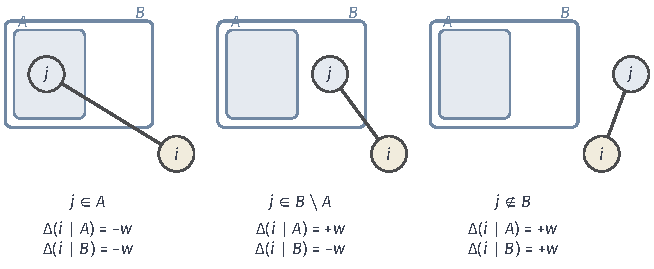
\includegraphics[width=110.723mm]{figures/01-basic-mathematics/04-graphs/tikz/c4-cut-submodular-cases/figure.pdf}
  \caption{割权函数次模性的逐边验证。固定一条权为$w\geq0$的边$\{i,j\}$，已选集合$A\subseteq B$（内框为$A$，外框为$B$），待加入的端点$i$（黄色）不在$B$中。按另一端点$j$的位置分三种情形：$j\in A$时两个增益都是$-w$；$j\in B\setminus A$时$A$上增益为$+w$、$B$上增益为$-w$；$j\notin B$时两个增益都是$+w$。每种情形都有$\Delta(i\mid A)\geq\Delta(i\mid B)$。}
  \label{fig:graph-setfn-cut-submodular-cases}
\end{figure}

\paragraph{次模与单调互不蕴含}
割权常常随集合增大而下降：$\operatorname{cut}(\varnothing)=\operatorname{cut}(V)=0$，而中间的子集可以有正的割权。图~\ref{fig:graph-setfn-property-counterexamples}(b)是只有一条权$1$的边的情形，割权依次为$0,1,1,0$，从单元素集到$\{1,2\}$时下降，所以次模函数不必单调。反方向，图~\ref{fig:graph-setfn-property-counterexamples}(a)的函数
\[
  F(S)=\max\bigl\{3\,\mathbb I\{\{1,2\}\subseteq S\},\ \mathbb I\{3\in S\}\bigr\}
\]
是单调的，但$\Delta(2\mid\varnothing)=0<3=\Delta(2\mid\{1\})$，违反式~\eqref{eq:graph-setfn-diminishing-returns}，所以单调函数也不必次模。

\begin{figure}[!htb]
  \centering
  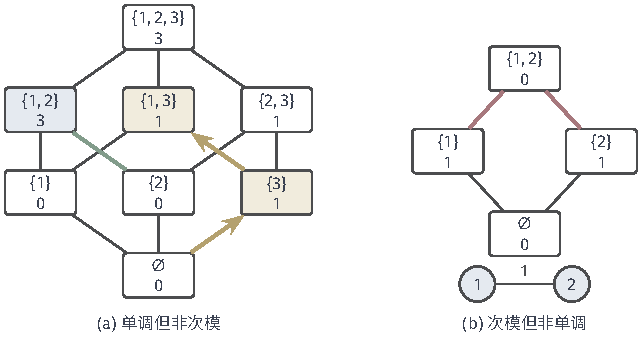
\includegraphics[width=108.687mm]{figures/01-basic-mathematics/04-graphs/tikz/c4-property-counterexamples/figure.pdf}
  \caption{单调性与次模性互不蕴含。每个框上行是子集，下行是函数值，连线连接只差一个元素的子集。(a) $F(S)=\max\{3\,\mathbb I\{\{1,2\}\subseteq S\},\mathbb I\{3\in S\}\}$：沿任一连线向上函数值不减，但绿色连线$\{2\}\to\{1,2\}$的增益$3$大于从空集加入$2$的增益$0$；黄色箭头是第~\ref{sec:graph-cardinality-selection}节贪心选择的路径，蓝色框是两元素时的最优集合。(b) 单条权$1$的边上的割权：次模，但红色连线上函数值从$1$降到$0$。}
  \label{fig:graph-setfn-property-counterexamples}
\end{figure}

\paragraph{超模性与协同}
把式~\eqref{eq:graph-setfn-diminishing-returns}的不等号反过来，即要求$\Delta(v\mid A)\leq\Delta(v\mid B)$，得到的函数称为\term{超模}函数（supermodular function）；等价地，$F$超模当且仅当$-F$次模。超模描述的是协同：两个部件只有同时具备才能工作时，单独加入任何一个的增益都是$0$，在另一个已经存在时加入，增益才是正的。例如$F(S)=\mathbb I\{\{1,2\}\subseteq S\}$是超模的。图~\ref{fig:graph-setfn-property-counterexamples}(a)的函数既不是次模也不是超模：元素$1,2$之间是协同的，而元素$3$与$\{1,2\}$之间是替代的，$\Delta(3\mid\varnothing)=1>0=\Delta(3\mid\{1,2\})$。

单调、模、次模、超模分别约束不同的东西，覆盖量、割权、净收益和上面的反例说明它们可以以各种方式组合出现。后面各节的算法保证都会同时写明目标是最大化还是最小化、函数是否单调、是否次模，以及约束是什么；只凭“次模”二字，并不能决定应当采用哪种方法。
